%************************************************
\section{Voltage to Calcium Transformation Enhances Direction Selectivity in \NoCaseChange{\textit{Drosophila}} T4 neurons}
%motion detectors is determined by the
%dynamics of their input elements]{The temporal tuning of the Drosophila
%motion detectors is determined by the
%dynamics of their input elements}
%\sectionmark{The temporal tuning of the Drosophila
%motion detectors is determined by the
%dynamics of their input elements}
\label{sct:manuscript_mishra_haag}
%************************************************


\paragraph{Abstract}
A critical step in neural information processing is the transformation of membrane voltage into calcium signals leading to transmitter release. However, the effect of voltage to calcium transformation on neural responses to different sensory stimuli is not well understood. Here, we use in vivo two-photon imaging of genetically encoded voltage and calcium indicators, Arclight and GCaMP6f respectively, to measure responses in \textit{Drosophila} direction-selective T4 neurons. Comparison between Arclight and GCaMP6f signals revealed calcium signals to have a significantly higher direction selectivity compared to voltage signals. Using these recordings we build a model which transforms T4 voltage responses to calcium responses. The model reproduces experimentally measured calcium responses across different visual stimuli using different temporal filtering steps and a stationary non-linearity. These findings provide a mechanistic underpinning of the voltage-to-calcium transformation and show how this processing step, in addition to synaptic mechanisms on the dendrites of T4 cells, enhances direction selectivity in the output signal of T4 neurons.


\paragraph{Authors} \textbf{Abhishek Mishra}, Alexander Borst, and Juergen Haag

\paragraph{Contributions}
Abhishek Mishra, Conceptualization, Investigation, Data curation, Software, Visualization, Writing original draft, review and editing; Juergen Haag, Conceptualization, Data curation, Software, Investigation, review and editing; Alexander Borst, Conceptualization, Funding acquisition, Project administration, Review and editing

\cleardoublepage

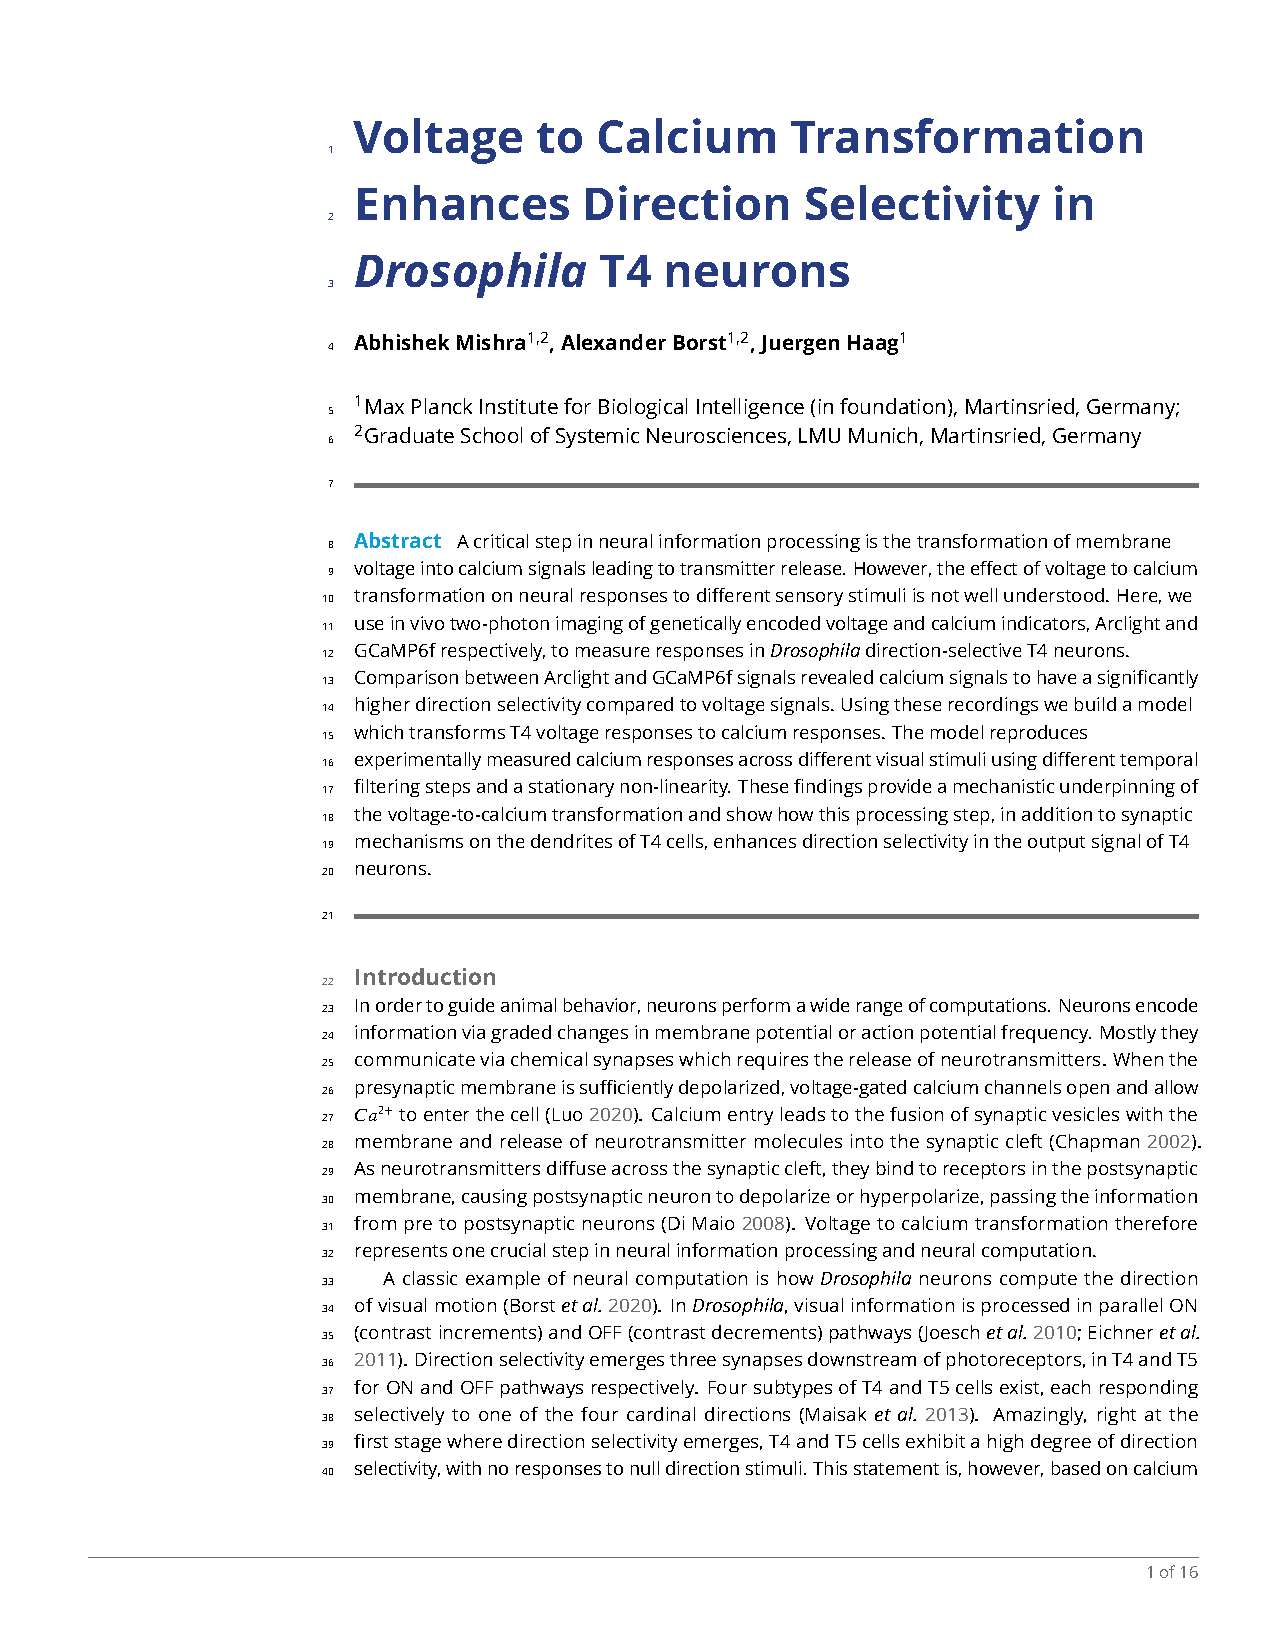
\includepdf[pages=-,scale=0.9,offset= 0 40,pagecommand={\thispagestyle{plain}}]{papers/Mishra_Haag_2022}